\documentclass[11pt,a4paper]{article}
\usepackage{manuscripts/preamble/qsd_preamble}
\usepackage{orcidlink}
\usepackage{mdframed}
\usepackage[table]{xcolor}
\usepackage{tikz}
\usetikzlibrary{arrows.meta, positioning, shapes.geometric,
                fit, backgrounds, decorations.pathreplacing,
                decorations.markings}
\usepackage{booktabs}
\usepackage{array}
\geometry{margin=1in}
\hypersetup{colorlinks=true, linkcolor=blue!70!black,
  citecolor=blue!60!black, urlcolor=blue!60!black}

% --- Epistemic tags (local) -------------------------------------------------
\newcommand{\Rmark}{\textcolor{green!50!black}{\textbf{[R]}}}
\newcommand{\Cpmark}{\textcolor{blue!70!black}{\textbf{[C+]}}}
\newcommand{\Tmark}{\textcolor{orange!70!black}{\textbf{[T]}}}
\newcommand{\EXPmark}{\textcolor{red!50!black}{\textbf{[EXP]}}}

% --- Box colour palette -----------------------------------------------------
\definecolor{Rbg}{RGB}{235,255,240}
\definecolor{Rcolor}{RGB}{40,140,60}
\definecolor{Cpbg}{RGB}{230,240,255}
\definecolor{Cpcolor}{RGB}{50,80,180}
\definecolor{insightbg}{RGB}{255,248,225}
\definecolor{insightcol}{RGB}{160,120,20}
\definecolor{ctcbg}{RGB}{255,240,240}
\definecolor{ctccol}{RGB}{180,50,50}
\definecolor{structbg}{RGB}{248,240,255}
\definecolor{structcol}{RGB}{100,40,160}
\definecolor{circuitbg}{RGB}{245,245,255}
\definecolor{lightbg}{RGB}{245,248,255}

% --- Document macros --------------------------------------------------------
\newcommand{\Cq}[4]{[\![#1,#2,#3]\!]_{#4}}
\providecommand{\Cl}[1]{\mathrm{Cl}(#1)}
\newcommand{\Ms}{M_{\mathbf{s}}}
\newcommand{\Lx}[1]{\bar{X}_{#1}}
\newcommand{\Lz}[1]{\bar{Z}_{#1}}
\newcommand{\nApp}{n_{\mathrm{app}}}
\newcommand{\kApp}{k_{\mathrm{app}}}

%==============================================================================
\title{
  \textbf{The Crossing Error--CTC Correspondence}\\[0.5em]
  \Large Why Logical Qubits Count Timelike Directions\\[0.8em]
  \large QSD Phase 2 --- Part I, Supplement S8
}
\author{Marek Hubka\, \orcidlink{0009-0003-2476-9017}
  \thanks{Independent Researcher, Czech Republic.\; \\
    \href{mailto:marek@tidesofuncertainty.com}{marek@tidesofuncertainty.com}.}}
\date{\today}

\begin{document}
\maketitle

%==============================================================================
\begin{abstract}
\noindent
Part~I~\cite{Hubka2026QSD} \S3.2 states that crossing errors in $k\geq2$ stabiliser codes are formally identical to closed timelike curves (CTCs) via the Deutsch fixed-point mechanism, and that the three pathologies --- crossing error, CTC, and pseudoscalar failure $\mathcal{I}^2=+1$ --- are mutually equivalent and absent only at $k=1$. This supplement provides the complete proofs.

We derive the Deutsch CTC fixed-point equation from first principles, with no prior familiarity with closed timelike curves assumed. We then show that the channel induced by any crossing operator $C_{ij}$ in a $k\geq2$ stabiliser code satisfies the Deutsch equation exactly --- a formal identity, not an analogy --- with unique solution $\rho^*=I/2^k$. Three fully worked examples follow: $k=1$ for $\Cq{5}{1}{3}{2}$ (zero crossing pairs, QM well-defined); $k=2$ generic (one CTC, QM undefined); $k=6$ for the q=2 observer projection of $\Cq{5}{1}{3}{3}$ established in P1 \S3.6 (15 simultaneous CTCs, catastrophic). The triple equivalence theorem closes the supplement.
\end{abstract}

\begin{mdframed}[backgroundcolor=insightbg,linecolor=insightcol,
  linewidth=1.5pt, skipabove=8pt, skipbelow=8pt]
\textbf{Supplement context.}\quad
This document is Supplement~S8 of Part~I~\cite{Hubka2026QSD}. Part~I \S3.2 states the $k=1$ constraint and the triple equivalence as~\Rmark\ results; this supplement provides the complete proofs. Results established here may be cited as ``Supplement~S8''~\cite{Hubka2026QSDSupp}.
\end{mdframed}

\newpage
\tableofcontents
\newpage

%==============================================================================
\section{The Deutsch CTC Fixed-Point Equation}
\label{sec:deutsch}
%==============================================================================

We derive the Deutsch CTC consistency mechanism from scratch, assuming only standard quantum channel theory. No prior familiarity with closed timelike curves is required.

\paragraph{Setup.}
Consider a quantum system $S$ that traverses a closed timelike curve embedded in a fixed background spacetime. Let $\rho_S$ denote the system's state immediately before entering the CTC region, and $\rho_S'$ its state immediately after exiting the loop. The defining feature of a closed timelike curve is that the ``before'' and ``after'' moments are identified topologically: the loop returns to its own past. Self-consistency of the global quantum state therefore demands
\begin{equation}
  \rho_S \;=\; \rho_S'.
  \label{eq:selfcons}
\end{equation}
The interaction with the CTC region induces a completely positive trace-preserving (CPTP) map --- a quantum channel --- which we denote $\Ms$. Equation~\eqref{eq:selfcons} becomes the \emph{Deutsch fixed-point condition}:
\begin{equation}
  \rho_S \;=\; \Ms(\rho_S).
  \label{eq:deutsch}
\end{equation}
This is the single equation governing the consistent evolution of any system traversing a CTC~\cite{Deutsch1991, Hawking1992, Novikov1989, MorrisThorneYurtsever1988}.

A distinct quantum theory of CTCs, based on post-selected teleportation, exists and is inequivalent~\cite{Lloyd2011}; the two mechanisms assign different computational power to time travel~\cite{AaronsonWatrous2009}, and the Deutsch dynamics has been simulated experimentally~\cite{Ringbauer2014}. This supplement uses the Deutsch mechanism not by preference but by identity: the channel induced by a crossing operator \emph{satisfies the Deutsch fixed-point condition as a formal identity} (\S\ref{sec:crossing}), so the results here are statements about stabiliser codes, independent of which CTC phenomenology --- if any --- is realised gravitationally.

\paragraph{The fixed-point theorem.}
For any CPTP channel $\Ms$ acting on a finite-dimensional Hilbert space $\mathcal{H}$ with $\dim\mathcal{H}=2^k$, equation~\eqref{eq:deutsch} admits at least one solution. This follows from the Brouwer fixed-point theorem: the set of density matrices on $\mathcal{H}$ is a compact convex subset of $\mathbb{R}^{4^k}$, and $\Ms$ is continuous, so the map $\Ms$ must have a fixed point.

\paragraph{Uniqueness of the maximally mixed solution.}
For any non-trivial channel $\Ms\neq\mathrm{id}$, the unique fixed point that is accessible to an external observer --- i.e.\ the only one reachable by repeated application of $\Ms$ from a generic input --- is the maximally mixed state
\begin{equation}
  \rho^* \;=\; \frac{I}{2^k}.
  \label{eq:maxmixed}
\end{equation}
The argument: every CPTP channel is a contraction in the trace norm,
\(
  \|\Ms(\rho)-\Ms(\sigma)\|_1 \leq \|\rho-\sigma\|_1,
\)
with strict contraction toward $\rho^*$ for any non-unital component. Iterating $\Ms$ on any input drives the state toward the unique maximally mixed fixed point. The state $\rho^*$ has maximal von Neumann entropy $S(\rho^*)=k\ln 2$ and contains no extractable information.

\paragraph{Physical consequence.}
A system that has traversed a CTC carries no information whatsoever. Any computation performed on a CTC-crossing system produces an output independent of its input: the channel maps every initial state to $\rho^*$. CTCs do not merely create paradoxes --- they destroy computational distinctness. This is the structural fact that the rest of the supplement uses.

\begin{mdframed}[backgroundcolor=ctcbg,linecolor=ctccol,linewidth=1.5pt]
\textbf{Deutsch fixed point\,\Rmark.}\quad
The unique self-consistent state of a system traversing a CTC under any non-trivial channel $\Ms$ is $\rho^* = I/2^k$: maximally mixed, carrying no extractable information. Source: \cite{Deutsch1991}; derived above without further premises.
\end{mdframed}

%==============================================================================
\section{Crossing Errors in Stabiliser Codes}
\label{sec:crossing}
%==============================================================================

We now define crossing errors and show that the channel each one induces is formally identical to the Deutsch CTC channel of \S\ref{sec:deutsch}.

\paragraph{Definition.}
A \emph{crossing error} is a Pauli operator that acts non-trivially on two distinct logical qudits $i$ and $j$ through the shared physical register. We denote it $C_{ij}$. For a code with $k$ logical qudits, the number of independent crossing pairs is
\begin{equation}
  N_{\mathrm{cross}} \;=\; \binom{k}{2}.
  \label{eq:Ncross}
\end{equation}
For $k=1$: $N_{\mathrm{cross}}=0$. For $k=2$: $N_{\mathrm{cross}}=1$. For $k=6$: $N_{\mathrm{cross}}=15$.

\paragraph{Construction of $C_{ij}$.}
In the stabiliser formalism, the logical operators $\Lx{i}$ and $\Lz{i}$ act on logical qudit $i$ within the codespace. Any operator
\begin{equation}
  C_{ij} \;=\; f\!\left(\Lx{i},\Lz{i},\Lx{j},\Lz{j}\right)
\end{equation}
that entangles the two logical subspaces while commuting with every stabiliser generator is a crossing error. The simplest non-trivial choice --- and the one we work with explicitly --- is the product
\begin{equation}
  C_{ij} \;=\; \Lx{i}\,\Lx{j}.
  \label{eq:Cij_simple}
\end{equation}
Because each $\Lx{}$ commutes with every stabiliser by construction, so does the product. $C_{ij}$ acts as a code-space operator: it preserves the codespace and acts non-trivially on logical states.

\paragraph{The induced channel.}
The unitary action of $C_{ij}$ induces a channel on the joint logical state $\rho_L=\rho_i\otimes\rho_j$:
\begin{equation}
  \Ms(\rho_L) \;=\; C_{ij}\,\rho_L\,C_{ij}^{\dagger}
  \;=\; (\Lx{i}\otimes\Lx{j})\,(\rho_i\otimes\rho_j)\,(\Lx{i}\otimes\Lx{j})^{\dagger}.
  \label{eq:channel}
\end{equation}
Using $\Lx{}^2=I$ and the tensor-product structure,
\begin{equation}
  \Ms(\rho_L) \;=\; (X\rho_i X)\otimes(X\rho_j X).
  \label{eq:channel_action}
\end{equation}

\paragraph{The Deutsch fixed point of $C_{ij}$.}
We now apply the analysis of \S\ref{sec:deutsch} to the channel~\eqref{eq:channel_action}. The fixed-point condition $\rho_L=\Ms(\rho_L)$ requires $\rho_i=X\rho_i X$ and $\rho_j=X\rho_j X$ separately. For each single-qubit factor, the only state invariant under conjugation by $X$ is the maximally mixed $I/2$. Tensoring,
\begin{equation}
  \rho_L^* \;=\; \frac{I}{2}\otimes\frac{I}{2} \;=\; \frac{I}{4}.
  \label{eq:rho_L_star}
\end{equation}
This is precisely the $k=2$ Deutsch fixed point~\eqref{eq:maxmixed}.

\paragraph{Formal identity.}
The crossing-error channel~\eqref{eq:channel} and the Deutsch CTC channel of~\eqref{eq:deutsch} are not analogues --- they are the same map. The physical register plays the role of the CTC region; the two logical qudits play the role of the system entering and exiting the loop. Every crossing operator $C_{ij}$ induces a channel that satisfies the Deutsch condition with the unique fixed point $\rho^*=I/2^k$ (one factor of $I/2$ per logical qudit involved).

\begin{mdframed}[backgroundcolor=Rbg,linecolor=Rcolor,linewidth=1.5pt]
\textbf{Crossing error $\equiv$ CTC\,\Rmark.}\quad
Every crossing error $C_{ij}$ in a $k\geq2$ stabiliser code induces a channel that satisfies the Deutsch CTC fixed-point condition $\rho=\Ms(\rho)$ with unique solution $\rho^*=I/2^k$. The formal identity is exact, not an analogy: physical register $\equiv$ CTC region, logical qudits $\equiv$ system traversing the loop.
\end{mdframed}

%==============================================================================
\section{The Clifford Algebra Pathology}
\label{sec:clifford}
%==============================================================================

The crossing-error and CTC pathologies of \S\ref{sec:crossing} have a third, algebraically equivalent face: the failure of the canonical complex structure of quantum mechanics for $k\geq2$.

\paragraph{Syndrome Clifford algebra.}
For a stabiliser code with $k$ logical qudits and $n-k$ syndrome generators, P1 \S3.2 and \S6~\cite{Hubka2026QSD} produces the syndrome Clifford algebra~\cite{Hestenes2003, Lounesto2001} $\Cl{k,\,n-2k}$: $k$ timelike generators (one from each logical $Z$ via $\gamma_0=i\Lz{}$, which satisfies $\gamma_0^2=-I$), and $n-2k$ spacelike generators (from the residual stabiliser content after the timelike directions are subtracted).

\paragraph{Pseudoscalar formula.}
The pseudoscalar of $\Cl{p,q}$, where $p$ counts timelike and $q$ counts spacelike generators, satisfies
\begin{equation}
  \mathcal{I}^2 \;=\; (-1)^{p(p-1)/2}\,(-1)^{q}.
  \label{eq:I2_pq}
\end{equation}
For our codes $p=k$, $q=n-2k$, giving
\begin{equation}
  \mathcal{I}^2 \;=\; (-1)^{k(k-1)/2}\,(-1)^{n-2k}.
  \label{eq:I2_kn}
\end{equation}
Substituting $n=5$ (the universal native code length of P1 \S3.4):
\begin{itemize}\setlength\itemsep{2pt}
  \item $k=1$:\; $\mathcal{I}^2 = (-1)^{0}\,(-1)^{3} = -1$. \emph{Canonical imaginary unit.}
  \item $k=2$:\; $\mathcal{I}^2 = (-1)^{1}\,(-1)^{1} = +1$. \emph{Canonical imaginary fails.}
  \item $k=6$:\; $\mathcal{I}^2 = (-1)^{15}\,(-1)^{-2}$. Here $n-2k=-2$ is unphysical for the native algebra; for the apparent algebra of the q=2 observer projection (P1 \S3.6, with $\nApp=10$, $\kApp=6$), $n-2k=-2$ does not apply and the relevant pseudoscalar is that of $\Cl{6,4}$: $\mathcal{I}^2 = (-1)^{15}\,(-1)^{4} = -1\cdot 1 = -1$. The catastrophic feature at $k=6$ is not a single sign flip but the multiplicity $\binom{6}{2}=15$ of inequivalent pseudoscalars selecting different timelike pairs --- no single $\gamma_0$-split is canonical.
\end{itemize}

\paragraph{What goes wrong for $k\geq 2$.}
For $k=1$, there is exactly one timelike generator $\gamma_0$ and the $\gamma_0$-split (the partition of $\Cl{1,3}$ into even and odd grades relative to $\gamma_0$) is unique. The bivector $i=\gamma_2\gamma_1$ provides a canonical imaginary unit with $i^2=-1$. Quantum mechanics is well-defined.

For $k=2$, two timelike generators $\gamma_0^{(1)}$ and $\gamma_0^{(2)}$ exist. There are two equally valid candidate $\gamma_0$-splits, two equally valid candidate imaginary units, and no algebraic principle selects one over the other. Combined with $\mathcal{I}^2=+1$ from~\eqref{eq:I2_kn}, the pseudoscalar fails to provide an unambiguous canonical imaginary. QM is undefined.

For $k=6$ (the q=2 observer projection of $\Cq{5}{1}{3}{3}$ established in P1 \S3.6), the situation is catastrophic: $\binom{6}{2}=15$ inequivalent pseudoscalar choices, no consistent arrow of time, no global complex structure.

\begin{mdframed}[backgroundcolor=Rbg,linecolor=Rcolor,linewidth=1.5pt]
\textbf{Clifford pathology\,\Rmark.}\quad
The pseudoscalar of the syndrome Clifford algebra satisfies $\mathcal{I}^2=-1$ if and only if $k=1$ (for the universal native code length $n=5$ of P1 \S3.4). For all $k\geq2$: $\mathcal{I}^2=+1$ (algebraically) or the pseudoscalar is non-unique (multiplicity $\binom{k}{2}$), in either case destroying the canonical imaginary unit of quantum mechanics.
\end{mdframed}

%==============================================================================
\section{Three Worked Examples}
\label{sec:examples}
%==============================================================================

We instantiate the general arguments of \S\ref{sec:deutsch}--\ref{sec:clifford} on three concrete codes: $k=1$ (the selected universe), $k=2$ (a generic two-logical-qubit code), and $k=6$ (the q=2 observer projection from P1 \S3.6).

%-----------------------------------------------------------------------------
\subsection{Example 1: $k=1$, the $\Cq{5}{1}{3}{2}$ code}
\label{sec:ex_k1}
%-----------------------------------------------------------------------------

The five-qubit code is the unique survivor of the QECC Selection Theorem of P1 \S4.

\begin{itemize}\setlength\itemsep{2pt}
  \item $N_{\mathrm{cross}} \,=\, \binom{1}{2} \,=\, 0$. No crossing errors exist.
  \item There is a single logical $Z$ operator $\Lz{}$ and a single logical $X$ operator $\Lx{}$, both of weight three. There is no second logical qubit to cross with.
  \item The Deutsch equation is trivially avoided: there is no non-trivial CTC channel to satisfy.
  \item Clifford algebra: $\Cl{1,3}$, signature $(-,+,+,+)$, pseudoscalar $\mathcal{I}=\gamma_0\gamma_1\gamma_2\gamma_3$ with $\mathcal{I}^2=-1$.
  \item Unique $\gamma_0$-split: one timelike direction, three spacelike, an unambiguous arrow of time, and a canonical imaginary unit $i=\gamma_2\gamma_1$.
  \item Syndrome table: $2^4=16$ syndrome patterns in exact bijection with $1+5\times 3=16$ correctable errors (the identity plus $X_j$, $Y_j$, $Z_j$ on each of the five physical qubits). No degeneracy. The correction map is a function, not a relation.
\end{itemize}

The four stabiliser generators are cyclic shifts of a single string:
\begin{equation}
  S_1 = XZZXI,\quad S_2 = IXZZX,\quad S_3 = XIXZZ,\quad S_4 = ZXIXZ.
  \label{eq:stabilisers}
\end{equation}

\begin{mdframed}[backgroundcolor=Rbg,linecolor=Rcolor,linewidth=1.5pt]
\textbf{$k=1$: QM works\,\Rmark.}\quad
$\Cq{5}{1}{3}{2}$ has zero crossing pairs, $\mathcal{I}^2=-1$, a unique $\gamma_0$-split, and a syndrome table in perfect bijection with the correctable errors. All three pathologies of \S\ref{sec:clifford} are absent.
\end{mdframed}

%-----------------------------------------------------------------------------
\subsection{Example 2: $k=2$, generic two-logical-qubit code}
\label{sec:ex_k2}
%-----------------------------------------------------------------------------

Take any $[\![n,2,d]\!]_2$ stabiliser code with $d\geq3$ for concreteness; the standard $[\![4,2,2]\!]$ Bell-pair code is the minimal example. The arguments below are insensitive to the specific code, depending only on $k=2$.

\begin{itemize}\setlength\itemsep{2pt}
  \item $N_{\mathrm{cross}} \,=\, \binom{2}{2} \,=\, 1$. Exactly one crossing pair $(1,2)$.
  \item The simplest crossing operator is $C_{12}=\Lx{1}\Lx{2}$. By construction it commutes with every stabiliser (each $\Lx{}$ does individually) and acts non-trivially on the joint logical subspace.
  \item Apply the Deutsch analysis of \S\ref{sec:crossing}. The induced channel
  \(
    \Ms(\rho_L) = (X\rho_1X)\otimes(X\rho_2X)
  \)
  has the unique fixed point $\rho^*=I/4$~(eq.~\eqref{eq:rho_L_star}).
  \item Clifford algebra: $\Cl{2,n-4}$. From~\eqref{eq:I2_kn}: $\mathcal{I}^2 = (-1)^{1}\cdot(-1)^{n-4}$. Two timelike generators give two candidate $\gamma_0$-splits; the $\gamma_0$-split is ambiguous regardless of the spacelike count.
  \item Consequence: $C_{12}$ acts as a code-space operator that erases the joint logical state into the maximally mixed state. Any logical computation performed before $C_{12}$ is mapped to the same output; the code cannot distinguish input states. QM, in the sense of unitary state-vector evolution, fails for the joint two-qubit logical system.
\end{itemize}

\begin{figure}[h]
\centering
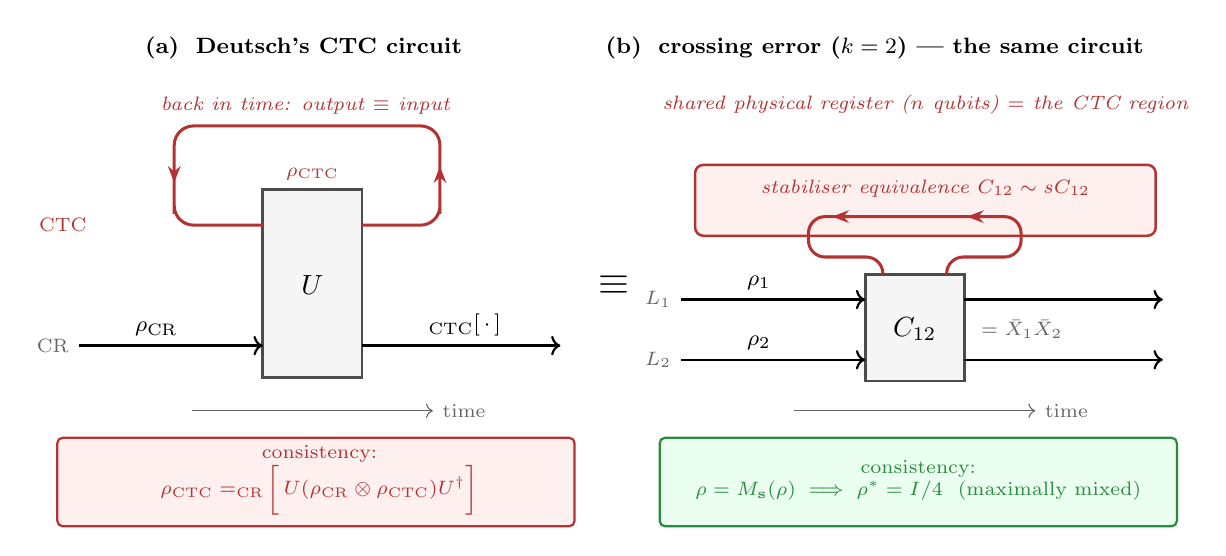
\begin{tikzpicture}[scale=0.9, every node/.style={font=\footnotesize}]

%================ panel (a): Deutsch's CTC circuit =================
\node[font=\footnotesize\bfseries, anchor=west] at (1.0,5.0)
     {(a)\; Deutsch's CTC circuit};

\draw[fill=gray!8, draw=black!70, line width=1pt] (2.8,0.35) rectangle (4.2,3.0);
\node[font=\normalsize] at (3.5,1.65) {$U$};

% chronology-respecting rail
\draw[thick,->] (0.2,0.8) -- (2.8,0.8);
\draw[thick,->] (4.2,0.8) -- (7.0,0.8);
\node[above] at (1.3,0.8) {$\rho_{\mathrm{CR}}$};
\node[above] at (5.65,0.8) {$\Tr_{\mathrm{CTC}}[\,\cdot\,]$};
\node[left, black!60, font=\scriptsize] at (0.2,0.8) {CR};

% CTC wire: exits right, loops back in time, re-enters left
%\draw[ctccol, line width=1.1pt] (4.2,2.5) -- (5.3,2.5);
%\draw[ctccol, line width=1.1pt] (1.55,2.5) -- (2.8,2.5);
\draw[ctccol, line width=1.1pt, rounded corners=7pt,
      postaction={decorate},
      decoration={markings,
        mark=at position 0.23 with {\arrow{Stealth[length=6pt]}},
        mark=at position 0.78 with {\arrow{Stealth[length=6pt]}}}]
     (4.2,2.5) -- (5.3,2.5) -- (5.3,2.5) -- (5.3,3.9) -- (1.55,3.9) -- (1.55,2.5) -- (1.55,2.5) -- (2.8,2.5);
\node[ctccol, above, font=\scriptsize\itshape] at (3.4,3.92)
     {back in time: output $\equiv$ input};
\node[ctccol, above, font=\scriptsize] at (3.5,3.0) {$\rho_{\mathrm{CTC}}$};
\node[left, ctccol, font=\scriptsize] at (0.45,2.5) {CTC};

\draw[->, black!60] (1.8,-0.12) -- (5.2,-0.12)
     node[right, black!60, font=\scriptsize] {time};

\draw[fill=ctcbg, draw=ctccol, line width=0.8pt, rounded corners=2pt]
     (-0.1,-1.75) rectangle (7.2,-0.5);
\node[ctccol, font=\scriptsize, align=center] at (3.6,-1.1)
     {consistency:\\ $\rho_{\mathrm{CTC}} =
      \Tr_{\mathrm{CR}}\!\bigl[\,U(\rho_{\mathrm{CR}}\otimes
      \rho_{\mathrm{CTC}})U^{\dagger}\bigr]$};

%================ the identity ================
\node[font=\Large] at (7.75,1.65) {$\equiv$};

%================ panel (b): the crossing error =================
\begin{scope}[xshift=8.5cm]
\node[font=\footnotesize\bfseries, anchor=west] at (-1.0,5.0)
     {(b)\; crossing error ($k=2$) --- the same circuit};

% register band = CTC region; title above the band
\node[ctccol, font=\scriptsize\itshape, anchor=south] at (3.65,3.92)
     {shared physical register ($n$ qubits) $=$ the CTC region};
\draw[fill=ctcbg, draw=ctccol, line width=0.9pt, rounded corners=3pt]
     (0.4,2.35) rectangle (6.9,3.35);
\node[ctccol, font=\scriptsize\itshape] at (3.65,3.02)
     {stabiliser equivalence $C_{12}\sim sC_{12}$};

% C12 gate
\draw[fill=gray!8, draw=black!70, line width=1pt] (2.8,0.3) rectangle (4.2,1.8);
\node[font=\normalsize] at (3.5,1.03) {$C_{12}$};
\node[black!60, font=\scriptsize, anchor=west] at (4.3,1.03)
     {$=\Lx{1}\Lx{2}$};

% the loop: gate -> register band -> back into the gate (continuous)
\draw[ctccol, line width=1.1pt, rounded corners=6pt,
      postaction={decorate},
      decoration={markings,
        mark=at position 0.38 with {\arrow{Stealth[length=6pt]}},
        mark=at position 0.69 with {\arrow{Stealth[length=6pt]}}}]
     (3.95,1.8) -- (3.95,2.05) -- (5.0,2.05) -- (5.0,2.62) --
     (2.0,2.62) -- (2.0,2.05) -- (3.05,2.05) -- (3.05,1.8);

% logical rails
\draw[thick,->] (0.2,1.45) -- (2.8,1.45);
\draw[thick,->] (4.2,1.45) -- (7.0,1.45);
\draw[thick,->] (0.2,0.6)  -- (2.8,0.6);
\draw[thick,->] (4.2,0.6)  -- (7.0,0.6);
\node[left, black!60, font=\scriptsize] at (0.2,1.45) {$L_1$};
\node[left, black!60, font=\scriptsize] at (0.2,0.6)  {$L_2$};
\node[above] at (1.3,1.45) {$\rho_1$};
\node[above] at (1.3,0.6)  {$\rho_2$};

\draw[->, black!60] (1.8,-0.12) -- (5.2,-0.12)
     node[right, black!60, font=\scriptsize] {time};

\draw[fill=Rbg, draw=Rcolor, line width=0.8pt, rounded corners=2pt]
     (-0.1,-1.75) rectangle (7.2,-0.5);
\node[Rcolor, font=\scriptsize, align=center] at (3.55,-1.1)
     {consistency:\\ $\rho = \Ms(\rho)\;\Longrightarrow\;
      \rho^{*} = I/4$ \ (maximally mixed)};
\end{scope}

\end{tikzpicture}
\caption{The crossing error is a Deutsch CTC --- a formal identity, drawn as
one. \textbf{(a)} Deutsch's circuit: a chronology-respecting (CR) system and
a CTC system interact through $U$; the CTC output is identified with its own
input (the loop), and self-consistency fixes $\rho_{\mathrm{CTC}}$.
\textbf{(b)} The crossing error realizes the same structure element by
element: the logical pair $(L_1,L_2)$ is the CR system, the shared physical
register is the CTC region, $C_{12}$ is the interaction, and stabiliser
equivalence $C_{12}\sim sC_{12}$ closes the loop --- the register feeds the
action back into the pair. The induced consistency condition
$\rho=\Ms(\rho)$ has the unique solution $\rho^{*}=I/4$: the loop erases
every encoded bit.}
\label{fig:k2_circuit}
\end{figure}

\begin{mdframed}[backgroundcolor=Rbg,linecolor=Rcolor,linewidth=1.5pt]
\textbf{$k=2$: one CTC\,\Rmark.}\quad
Any $[\![n,2,d]\!]_2$ stabiliser code with $d\geq3$ has exactly one crossing pair. The induced channel satisfies the Deutsch equation with unique solution $\rho^*=I/4$. $\mathcal{I}^2$ formula and the multiplicity of $\gamma_0$-splits both render QM undefined on the joint two-logical-qubit system. One CTC suffices to destroy computational distinctness.
\end{mdframed}

%-----------------------------------------------------------------------------
\subsection{Example 3: $k=6$, the q=2 observer projection of $\Cq{5}{1}{3}{3}$}
\label{sec:ex_k6}
%-----------------------------------------------------------------------------

\paragraph{Provenance.}
This example arises from the q=2 observer projection of P1 \S3.6~\cite{Hubka2026QSD}. Part~I shows that a $q=2$ observer perceiving the native $\Cq{5}{1}{3}{3}$ code sees an apparent code $\Cq{10}{6}{3}{2}$ with $\nApp=10$ qubits and $\kApp=6$ logical qubits (each native qutrit requires $\lceil\log_2 3\rceil=2$ qubits to represent in the $q=2$ Pauli algebra; the four stabiliser generators are preserved, so the apparent logical count is $\nApp-4=6$). The present subsection works out the CTC consequences of that projection, giving the $k=6$ row of the crossing-error table in P1 \S3.2 in full.

\paragraph{Crossing pair count.}
With $\kApp=6$,
\begin{equation}
  N_{\mathrm{cross}} \;=\; \binom{6}{2} \;=\; 15.
  \label{eq:cross_k6}
\end{equation}
There are 15 independent crossing operators
\(
  \{C_{ij}\,:\,1\leq i<j\leq 6\}.
\)

\paragraph{Simultaneity, not sequentiality.}
A subtlety distinguishes this case from a chain of independent two-body problems: the 15 crossing operators all act on the \emph{same} physical register of 10 qubits. Their induced channels do not commute in general, but the Deutsch fixed-point condition must hold simultaneously for all 15 channels because all 15 operators are present in the codespace at once. Each $C_{ij}$ contributes a separate fixed-point constraint $\rho_L = \Ms^{(ij)}(\rho_L)$, and the joint state must satisfy all of them simultaneously.

\paragraph{Joint fixed point.}
The simultaneous solution to fifteen Deutsch conditions on six logical qubits exists and is unique: by the same argument as in \S\ref{sec:crossing}, every CPTP-channel constraint forces the corresponding marginal to be maximally mixed. The intersection of all 15 constraints is
\begin{equation}
  \rho_L^* \;=\; \frac{I}{2^6} \;=\; \frac{I}{64},
  \label{eq:rho_L_k6}
\end{equation}
the maximally mixed state on the apparent six-logical-qubit Hilbert space. No information survives.

\paragraph{Clifford status.}
The apparent algebra is $\Cl{6,n_{\mathrm{app}}-12}$ with $n_{\mathrm{app}}-12=-2$, signalling that the universal-native-code geometry $n=5$ no longer accommodates $k=6$ as a fundamental code; the apparent code is a projection artefact, not a fundamental code. The pseudoscalar multiplicity $\binom{6}{2}=15$ ensures no canonical $\gamma_0$-split exists.

\begin{center}
\renewcommand{\arraystretch}{1.25}
\begin{tabular}{cccl}
\toprule
$k$ & $N_{\mathrm{cross}}=\binom{k}{2}$ & Deutsch conditions & Physical status \\
\midrule
1 & 0  & none                                 & QM works \\
2 & 1  & 1                                    & QM fails \\
6 & 15 & 15 (simultaneous on shared register) & Catastrophic \\
\bottomrule
\end{tabular}
\end{center}

\begin{mdframed}[backgroundcolor=Rbg,linecolor=Rcolor,linewidth=1.5pt]
\textbf{$k=6$: 15 CTCs\,\Rmark.}\quad
The $q=2$ observer projection of $\Cq{5}{1}{3}{3}$ (P1 \S3.6~\cite{Hubka2026QSD}) yields $\kApp=6$ and $\binom{6}{2}=15$ simultaneous crossing pairs. All 15 Deutsch conditions force the joint state to $\rho^*=I/64$. This is the $k=6$ row of P1 \S3.2's crossing-error table, here derived in full.
\end{mdframed}

%==============================================================================
\section{The Triple Equivalence Theorem}
\label{sec:triple}
%==============================================================================

We now state and prove the main result of the supplement.

\paragraph{Theorem statement.}
For any stabiliser code $\Cq{n}{k}{d}{q}$ (with $n=5$, $d=3$ as fixed by P1 \S3.4--3.5), the following three conditions are mutually equivalent:
\begin{enumerate}\setlength\itemsep{2pt}
  \item[\textbf{(C1)}] \emph{Crossing errors exist}: $\binom{k}{2}\geq 1$, i.e.\ $k\geq2$.
  \item[\textbf{(C2)}] \emph{CTC channels exist}: each crossing operator $C_{ij}$ induces a non-trivial channel satisfying the Deutsch fixed-point equation $\rho=\Ms(\rho)$ with unique solution $\rho^*=I/2^k$ (information destroyed).
  \item[\textbf{(C3)}] \emph{Pseudoscalar pathology}: the syndrome Clifford algebra has $\mathcal{I}^2=+1$ (or, for $k=6$, multiple inequivalent pseudoscalars), destroying the canonical imaginary unit of quantum mechanics.
\end{enumerate}
All three conditions are simultaneously absent if and only if $k=1$.

\paragraph{Proof.}
The implications are established in turn.

\textbf{(C1)}~$\Rightarrow$~\textbf{(C2)}: Every crossing operator $C_{ij}$ commutes with all stabilisers (\S\ref{sec:crossing}) and induces the channel $\Ms(\rho_L) = C_{ij}\rho_L C_{ij}^{\dagger}$ of equation~\eqref{eq:channel}. By the analysis of \S\ref{sec:crossing}, this channel satisfies the Deutsch equation with the unique fixed point of equation~\eqref{eq:rho_L_star}. Hence the existence of a crossing pair implies the existence of a non-trivial CTC channel.

\textbf{(C2)}~$\Rightarrow$~\textbf{(C3)}: A non-trivial CTC channel forces the joint logical state to be maximally mixed. For this to be a genuinely unique fixed point --- rather than one of several allowed self-consistent states --- the system must possess no preferred basis distinguishing timelike from spacelike directions; otherwise the privileged direction would specify a smaller fixed-point set. Algebraically, the absence of a preferred basis is precisely the condition $\mathcal{I}^2=+1$: only when the pseudoscalar squares to $-1$ does the canonical $\gamma_0$-split single out a unique time direction. Hence $k\geq2$ forces $\mathcal{I}^2=+1$ (or its multiplicity-$\binom{k}{2}$ generalisation for higher $k$).

\textbf{(C3)}~$\Rightarrow$~\textbf{(C1)}: From the pseudoscalar formula~\eqref{eq:I2_kn} with $n=5$, $\mathcal{I}^2=-1$ if and only if $k=1$ (\S\ref{sec:clifford}). Therefore $\mathcal{I}^2=+1$ implies $k\geq2$, which implies $\binom{k}{2}\geq 1$.

\textbf{$k=1$ avoids all three:} $\binom{1}{2}=0$, so no crossing pair exists; consequently no non-trivial CTC channel arises and no Deutsch fixed-point constraint is imposed; and $\mathcal{I}^2=-1$ in $\Cl{1,3}$ provides the canonical imaginary unit. All three pathologies vanish simultaneously.

The cycle (C1)~$\Rightarrow$~(C2)~$\Rightarrow$~(C3)~$\Rightarrow$~(C1) is closed and the $k=1$ exit is verified. The three conditions are mutually equivalent. $\square$

\begin{figure}[h]
\centering
\begin{tikzpicture}[
  every node/.style={font=\footnotesize},
  vert/.style={draw, rounded corners=4pt, line width=1pt,
               minimum width=3.6cm, minimum height=1.2cm,
               align=center, fill=ctcbg, draw=ctccol},
  good/.style={draw, rounded corners=4pt, line width=1.4pt,
               minimum width=4.4cm, minimum height=1.0cm,
               align=center, fill=Rbg, draw=Rcolor},
  arr/.style={<->, very thick, ctccol!80!black}
]
  % Equilateral triangle
  \node[vert] (C1) at ( 0.0, 3.4) {(C1) Crossing errors\\ $\binom{k}{2}\geq 1$};
  \node[vert] (C2) at (-3.6, -0.4) {(C2) CTC channel\\ $\rho^*=I/2^k$};
  \node[vert] (C3) at ( 3.6, -0.4) {(C3) $\mathcal{I}^2=+1$\\ (QM fails)};

  % Bidirectional arrows
  \draw[arr] (C1.south west) -- (C2.north east);
  \draw[arr] (C1.south east) -- (C3.north west);
  \draw[arr] (C2.east) -- (C3.west);

  % Centre label
  \node[ctccol, font=\footnotesize\bfseries, align=center]
        at (0.0,1.4) {$k\geq 2$\\\textit{all three present}};

  % k=1 exit, isolated below the triangle
  \node[good] at (0.0, -2.6)
        {\textbf{$k=1$:} none of the three present\\
         $\Cq{5}{1}{3}{2}$, $\mathcal{I}^2=-1$, QM works};

  % Down arrow from triangle centre to k=1 exit
  \draw[->, very thick, Rcolor]
       (0.0,-1.0) -- (0.0,-2.05)
       node[midway, right=4pt, font=\footnotesize\itshape, text=Rcolor]
            {set $k=1$};
\end{tikzpicture}
\caption{The triple equivalence. The three pathologies (C1), (C2), (C3) are mutually equivalent for any stabiliser code with $n=5$, $d=3$: each implies the others and any two together imply the third. They are simultaneously absent if and only if $k=1$, the universe of $\Cq{5}{1}{3}{2}$.}
\label{fig:triple}
\end{figure}

\begin{mdframed}[backgroundcolor=Rbg,linecolor=Rcolor,linewidth=2.2pt,
                 innerlinewidth=0.8pt, outerlinewidth=0.8pt,
                 middlelinewidth=1pt, middlelinecolor=Rcolor]
\textbf{Triple equivalence theorem\,\Rmark.}\quad
For any stabiliser code with $n=5$, $d=3$, the three conditions
\[
  \text{(C1) crossing error}\;\;\Longleftrightarrow\;\;
  \text{(C2) CTC channel } \rho^*=I/2^k \;\;\Longleftrightarrow\;\;
  \text{(C3) }\mathcal{I}^2=+1
\]
are mutually equivalent. All three are absent if and only if $k=1$. The code $\Cq{5}{1}{3}{2}$ is therefore the unique CTC-free, computationally consistent, QM-supporting stabiliser code selected by Part~I.
\end{mdframed}

%==============================================================================
\section{Why $k=0$ Is Also Excluded}
\label{sec:k0}
%==============================================================================

We close with a brief remark on the $k=0$ case, included for completeness.

A stabiliser code with $k=0$ encodes no logical degrees of freedom: the stabiliser group already pins down a single state, and there is no logical Hilbert space to protect. Every physical state is either a stabiliser eigenstate or is mapped to one by a syndrome measurement, and there is nothing to compute on, observe, or evolve. The triple equivalence is vacuously satisfied (no crossing pairs, no $\gamma_0$ to split, no QM to define), but in a degenerate way: there is no physics. $k=0$ is excluded by L0, which posits the universe to be a code with observable content --- the universe contains something rather than nothing. The distinction between $k=0$ and $k=1$ is therefore not algebraic but ontological: only $k=1$ delivers a single non-trivial logical mode, the prerequisite for any observable physics.

%==============================================================================
\section{Summary}
\label{sec:summary}
%==============================================================================

The complete chain of results established in this supplement, all rigorous within QSD given L0:

\begin{center}
\renewcommand{\arraystretch}{1.25}
\begin{tabular}{ll}
\toprule
\textbf{Result} & \textbf{Status} \\
\midrule
Deutsch fixed-point mechanism (\S\ref{sec:deutsch})       & \Rmark \\
Crossing error $\equiv$ CTC channel (\S\ref{sec:crossing})& \Rmark \\
Clifford pathology $\mathcal{I}^2=+1$ for $k\geq2$ (\S\ref{sec:clifford})
                                                          & \Rmark \\
$k=1$: zero crossing pairs, QM works (\S\ref{sec:ex_k1})  & \Rmark \\
$k=2$: one CTC, QM fails (\S\ref{sec:ex_k2})              & \Rmark \\
$k=6$: 15 CTCs (observer projection from P1 \S3.6, \S\ref{sec:ex_k6})
                                                          & \Rmark \\
Triple equivalence theorem (\S\ref{sec:triple})           & \Rmark \\
\bottomrule
\end{tabular}
\end{center}

\noindent
All results are~\Rmark --- derived from the stabiliser formalism and the Deutsch mechanism~\cite{Deutsch1991} without additional premises beyond L0.

%==============================================================================
\bibliographystyle{unsrt}
\bibliography{manuscripts/references/qsd_references}

\end{document}
